\newcommand{\institut}{}
\newcommand{\fachgebiet}{Halbleiterbauelemente}
\newcommand{\veranstaltung}{Praktikum Technologie und Bauelemente der Halbleitertechnik}
\newcommand{\pdfautor}{Dirk Barbendererde (321 836), Thomas Kapa (), Alona
Siebert (), Özgü Dogan (326048)}
\newcommand{\autor}{Dirk Barbendererde (321 836)\\ Thomas Kapa ()\\ Alona
Siebert ()\\ Özgü Dogan (326 048)}
\newcommand{\pdftitle}{Praktikum\ Technologie und Bauelemente der
Halbleitertechnik}
\newcommand{\prototitle}{Praktikum Technologie und Bauelemente der Halbleitertechnik}
\newcommand{\aufgabe}{}

\newcommand{\gruppe}{Gruppe 1}
\newcommand{\betreuer}{Betreuer:\\ Clemens Helfmeier\\ Philipp Scholz}



\input{../../packages/tu_header_9}

\setcaptionwidth{7.5cm}

\begin{document}


%     \lstinputlisting{./praktikum6.sce}



%---------------------------------------------------------------------
%---------------------------------------------------------------------
%---------------------------------------------------------------------

\section{Kennlinie}
\begin{quote}
    
    Benennung der Dateien:\\
    Kennlinie_{Wavernummer}_Die_[{Zeile},{Spalte}]_Mess_{messung}.mat\\
    
    100 µA Strombegrenzung\\
    Welche Diode?
    Welcher Manipulator
    
    SMU1 = GND
    SMU2 = GND
    SMU3 = Var1
    
    Unterdiffusion
    
    unterspannung
    0.0 & 2.4
    0.5 & 3.8
    0.8 & 4.5
    1.0 & 5.0
    1.3 & 5.5
    1.8 & 6.7
    2.5 & 8.2
    3.0 & 9.2
    
    \TODO{müssen wir die Dies durchnummerieren?}
\end{quote} %sec Kennlinie

%--------------------------------------------------------------------
%--------------------------------------------------------------------

\section{Schaltverhalten}
\begin{quote}
    
\end{quote} %sec Schaltverhalten

%--------------------------------------------------------------------
%--------------------------------------------------------------------

\section{Emissionsmessung}
\begin{quote}
    
    \TODO{Einleitung, Theorie, Verknüpfung, Messung, Ergebnisse, Auswertung}
    
    Eine Emissionsmessung ist in der Halbleitertechnologie insofern interessant,
    weil sie Erkenntnisse über charakteristische Eigenschaften des Halbleiters,
    in unserem Fall die selbst hergestellte Diode, liefert. Dazu gehören die
    Ladungsträgerlebensdauer $\tau_{n,p}$ und die Diffusionslänge $L_{n,p}$. Auf
    die Lebensdauer lässt sich mithilfe der Diffusionslänge und des
    Diffusionskoeffizienten schließen. Dieser ist ein materialabhängiger Wert,
    welcher von uns nicht weiter beachtet wird. Der folgende Zusammenhang hilft
    bei der Berechnung von $\tau_{n,p}$:
    
    \begin{equation*}
        \begin{split}
            L_{n,p} = \sqrt{\tau_{n,p} \cdot D_{n,p}} 
        \end{split}
    \end{equation*}
    
    Ziel unserer Messung aber, war die Bestimmung der Diffusionslänge in unserer
    Diode. Dieser wurde über die realisierte Intensitätsmessung anhand der
    Emissionen in der Diode ermittelt. Dabei wurden folgende
    Proportionalitätsverhätnisse verwendet:
    
    \begin{equation*}
        \begin{split}
            I(x) \sim \ \Delta n \sim \ exp(-\frac{x}{L_n}) 
        \end{split}
    \end{equation*}
    
    Hierbei werden Strahlungsintensität ins Verhältnis mit der\\
    Minoritätsüberschussladungträgerkonzentration, hier frei bewegliche
    Elektronen im p-Gebiet, und dieser wiederum ins Verhältnis mit einem
    Exponentialtherm gesetzt. Daher kann man die Intensitätsmessung direkt mit
    diesem Therm in Verbindung setzen, welcher in seinem Argument die gesuchte
    Diffusionslänge beinhaltet. Weiteres zur Berechnung des $L_n$ steht in der
    Auswertung der Messung.\\
    
    Um aber die Intensitätsmessung verstehen zu können müssen einige
    grundlegende Theorien der Halbleiter bezüglich ihrer Typen und ihrer
    Rekombinationsarten behandelt und nachvollzogen werden.\\ 
    Daher gibt es vor der Versuchsdurchführung und der Auswertung zunächst eine
    kleine Exkursion in den theoretischen Bereich.
    
        \subsection{Direkter und indirekter Halbleiter }
        \begin{quote}
        
        Es gibt zwei Arten von Halbleitern, die direkten und die indirekten
        Halbleiter. Diese unterscheiden sich darin, dass die Rekombination eines
        Ladungsträgers aus dem Leitungs- in das Valenzband unterschiedliche
        Vorraussetzungen erfordert.
            
            \subsubsection{direkter Halbleiter}
            \begin{quote}
            Die Rekombination bei einem direkten Halbleiter ist relativ simpel.
            Ein freies Elektron braucht dabei nur, unter Abgabe der jeweiligen
            Energie, den Bandabstand zwischen Leitungs- und Valenzband zu
            überqueren.
            
            \begin{figure}[H]
                    \centering
                        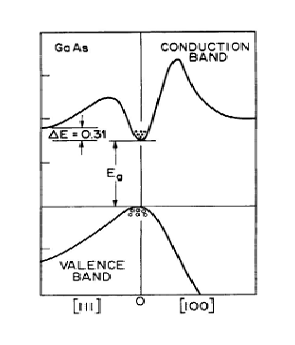
\includegraphics[scale=0.72, trim = 1cm 1cm 1.5cm 0cm,
                        clip]{./Emissionsbilder/restliches/direkt.png}
                        \caption{Rekombination bei einem direkten Halbleiter}
                            \label{fig:./Emissionsbilder/restliches/direkt.png}
            \end{figure}
            
            
            \end{quote}       
        
            \subsubsection{indirekter Halbleiter}
            \begin{quote}
            Die Rekombination bei einem indirekten Halbleiter erfordert neben
            einem Energieunterschied auch einen Impulsunterschied, damit das
            Elektron auf dem Valenzband auftreffen kann. Dieser
            Impulsunterschied ist in der folgenden Abbildung zu erkennen.
            
            \begin{figure}[H]
                    \centering
                        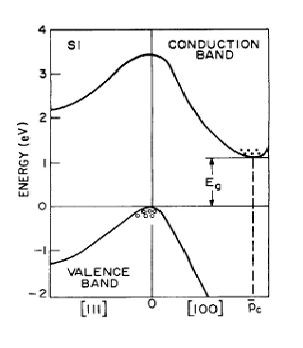
\includegraphics[scale=0.73, trim = 1cm 1cm 1.5cm 0cm,
                        clip]{./Emissionsbilder/restliches/indirekt.png}
                        \caption{Rekombination bei einem indirekten Halbleiter}
                            \label{fig:./Emissionsbilder/restliches/indirekt.png}
            \end{figure}
            
            \TODO{Bildquellen, TBH-Skript S.92 einfügen}
            \end{quote}       
            
            Ein weiterer Unterschied zwischen direkten und indirekten
            Halbleitern ist der, dass direkte Halbleiter hauptsächlich
            strahlend Rekombinieren, wohingegen indirekte Halbleiter
            stochastisch betrachtet fast nur nichtstrahlend Rekombinieren.
            Dennoch findet mit sehr geringer Wahrscheinlichkeit auch vereinzelt
            strahlende Rekombination in den indirekten Halbleitern statt.\\
            Bevor weiter darauf eingegangen wird, in wie fern dies für die
            Emissionsmessung von Bedeutung ist, werden die Rekombinationsarten,
            strahlend und nichtstrahlend, wiederholt.
            
        \end{quote}
        
        \subsection{Rekombinationsmechanismen}
        \begin{quote}
        
        Eine Rekombination erfolgt stets unter Abgabe von einer
        Energiedifferenz. Dabei wird unterschieden, ob diese Energie in Form
        eines Lichtquants oder von Wärme abgegeben wird, wodurch auch die
        Beschreibung strahlend oder nichtstrahlend entsteht.\\
        Nun folgen je ein Beispiel für diese Machanismen.
        
            \subsubsection{strahlende Rekombination}
            \begin{quote}
            
            Die strahlende Rekombination, hauptsächlich bei direkten Halbleitern
            zu sehen, besagt, dass der rekombinierende Ladungsträger die
            Energiedifferenz, welche er zurücklegt, in Form eines Photons
            freigibt. Die Energie dieses Photons beträgt genau die Energie des
            Bandabstands zwischen den beiden Bändern. Anders ausgedrückt kann
            man sie auch Rekombinationsenergie nennen:
                    
            \begin{equation*}
                \begin{split}
                    W_{Rek} = h \cdot \nu 
                \end{split}
            \end{equation*}
            
            Diese Rekombinationsenergie setzt sich aus des Produkt aus dem
            Planckschen Wirkungsquantums $h$ und die Frequenz des entstehenden
            Lichts $\nu$.\\
            
            Ein Beispiel für die strahlende Rekombination ist die
            Band-Band-Rekombination, welche in der folgenden Abbildung
            dargestellt wurde:
            
            \begin{figure}[H]
                    \centering
                        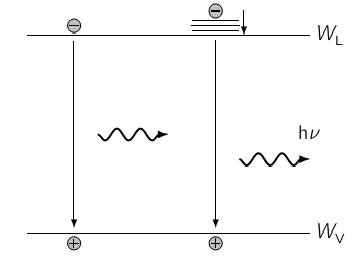
\includegraphics[scale=0.72, trim = 1cm 1cm 1.5cm 0cm,
                        clip]{./Emissionsbilder/restliches/bandband.png}
                        \caption{strahlende Band-Band-Rekombination}
                            \label{fig:./Emissionsbilder/restliches/direkt.png}
            \end{figure}
            
            Man erkennt ein Elektron, welches beim Rekombinieren, die bereits
            erwähnte Rekombinationsernergie in Form eines Photons abgibt. Es
            kann aber auch vorkommen, dass die abgegebene Energie an ein
            weiteres Eektron im Leitungsband abgegeben wird, wodurch dieser auf
            ein höheres Energieniveau im Leitungsband angehoben und wieder runterfallen 
            kann. Diese Möglichkeit ist bei der strahlenden Rekombination die
            unwarscheinlichere Variante.
            
            \end{quote}
            
            \subsubsection{nichtstrahlende Rekombination}
            \begin{quote}
            
            Die nichtstrahlende Rekombination findet hauptsächlich bei
            indirekten Halbleitern statt. Dabei wird die Rekombinationsenergie
            an ein weiteres Elektron im Leitungsband abgegeben, welches auf ein
            höheres Energieniveau angehoben wird und unter Abgabe von
            thermischer Energie wieder runterfallen kann.\\
            Als ein Beispiel für die nichtstrahlende Rekombination wird die
            Augerrekombination dargestellt:
            
            \begin{figure}[H]
                    \centering
                        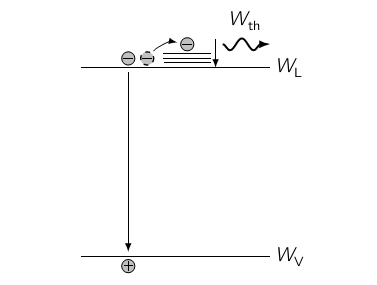
\includegraphics[scale=0.72, trim = 1cm 1cm 1.5cm 0cm,
                        clip]{./Emissionsbilder/restliches/auger.png}
                        \caption{nichtstrahlende Auger-Rekombination}
                            \label{fig:./Emissionsbilder/restliches/auger.png}
            \end{figure}
            
            \end{quote}
        
        Die für die Emissiosmessung verwendete Diode besteht aus Silizium,
        welcher ein indirekter Halbleiter ist und dessen Rekombinationen
        hauptsächlch nichtstrahlend ist. Wie aber schon bei den Halbleitertypen
        erwähnt, kann es bei indirekten Halbleitern auch mit sehr geringer
        Wahrscheinlichkeit zu strahlender Rekombination kommen. Da die Abgabe
        von thermischer Energie zu einem Temperaturunterschied in der Diode
        führen würde, bräuchte man bei den Emissionsmessung sehr feine und genau
        Thermometer, welche im $\mu m$-Bereich nicht realisierbar sind. Daher
        wird die stochastisch in geringer Menge vorhandene strahlende
        Rekombination betrachtet um über die mit lichtempfindlichen
        Kameras gemessene Lichtintensitäten auf die gesuchte Diffusionslänge
        schließen zu können.
        \end{quote}
    
    
    
    
\end{quote} %sec Emissionsmessung

%--------------------------------------------------------------------
%--------------------------------------------------------------------


\end{document}
